\documentclass[11pt,a4paper]{article}

\usepackage[utf8]{inputenc}
\usepackage[T1]{fontenc}
\usepackage{amsmath,amssymb}
\usepackage{geometry}
\usepackage{booktabs}
\usepackage{listings}
\usepackage{pgfplots}
\usepackage[colorlinks=true,linkcolor=blue,citecolor=blue,urlcolor=blue]{hyperref}

\geometry{left=2.5cm,right=2.5cm,top=2.5cm,bottom=2.5cm}
\pgfplotsset{compat=1.18}

\lstset{
  basicstyle=\ttfamily\small,
  breaklines=true,
  frame=single,
  numbers=left,
  numberstyle=\tiny,
  tabsize=2
}

\title{\textbf{NRR-Coupled (cp): Dependency-Consistency Evaluation for Coupled State Updates}}
\author{Kei Saito\thanks{ORCID: 0009-0006-4715-9176}\\Independent Researcher, Japan\\\texttt{kei.saito.research@gmail.com}}
\date{February 2026\\[0.5em]\textit{Part of the Non-Resolution Reasoning (NRR) research program.}}

\begin{document}
\maketitle

\begin{center}
\textcopyright\ 2026 Kei Saito. Licensed under CC BY 4.0.\\
\url{https://creativecommons.org/licenses/by/4.0/}
\end{center}

\begin{abstract}
This paper evaluates NRR-Coupled (cp), a client-side extension of Transfer-style updates for dependent-candidate conditions. The LLM interface is fixed (\((\sigma/\delta,\text{target})\)); only deterministic client propagation is varied. We compare uncoupled baseline (\(\beta=0\)) and coupled variants (\(\beta\in\{0.1,0.3,0.5\}\)) using 15 seed-fixed random operator streams for each of 3 patterns (\(n=4,5,6\)), with 12 turns per stream. Main metrics are (i) turn-wise dependency-consistency violation rate and (ii) additional repair operators needed after a primary-target stream. At \(\beta=0.3\), coupled updates reduce violation rate in D-dependent by 0.2123 and reduce repair operations by 0.58 on average, while D-mismatch increases violation rate by 0.2302 and repair operations by 3.31. D-independent remains exactly equivalent under strict numerical tolerance \(10^{-12}\), and its edge-based violation metric is structurally uninformative because \(A_{\text{eval}}=0\) yields zero evaluation opportunities. The results support a bounded claim: cp is beneficial when dependency structure is directionally correct and harmful when dependency signs are mis-specified.
\end{abstract}

\noindent\textbf{Keywords:} NRR-Coupled, dependency consistency, repair cost, falsifiable simulation, robustness

\section{Introduction}
This paper is one module in an ongoing Non-Resolution Reasoning (NRR) research program, not a closed endpoint. Companion papers cover foundational theory, text-to-state mapping, implementation behavior, and cross-domain transfer with distinct scopes.

LLM APIs are stateless across calls, while many applications require state updates over dependent candidates. NRR-Transfer addressed independent-candidate updates; cp extends client execution to dependent settings.

NRR is not an anti-LLM framework.
NRR does not replace standard LLM use.
NRR optimizes when to commit and when to defer, under explicit conditions.

\textbf{Boundary.}
Transfer: independent-candidate condition.
cp: dependent-candidate condition.
Uncoupled baseline is inherited from Transfer and not redefined.

Series Consistency Statement: Unsupported interpretations are never injected at a fixed evidence state. Hypothesis-set expansion is evidence-gated, and unobserved possibilities remain unresolved. Evidence in this paper is restricted to fixed simulation inputs and declared dependency structures.

\subsection{Contributions}
\begin{enumerate}
  \item We define a coupled client-side update extension for dependent-candidate conditions while keeping the LLM interface fixed at \((\sigma/\delta,\text{target})\).
  \item We provide a falsifiable simulation protocol that compares coupled and uncoupled execution under identical operator streams.
  \item We report bounded utility with explicit failure boundaries: gains under directionally correct dependencies and degradation under sign-mismatched dependencies.
\end{enumerate}

\section{Update Rule and Complexity}
Let \(\mathbf{w}_t\in\mathbb{R}^n\), \(\sum_i w_t^{(i)}=1\), and dependency matrix \(A\in\mathbb{R}^{n\times n}\), where \(A_{ij}\) is influence from candidate \(j\) to \(i\).

Given \((o_t,k_t)\) with \(o_t\in\{\sigma,\delta\}\):
\[
\Delta_t = +\alpha\;(\sigma),\ -\alpha\;(\delta),\qquad
\tilde{w}^{(k_t)}=\operatorname{clip}(w_t^{(k_t)}+\Delta_t,\varepsilon,u_{\max}).
\]
Here, \(+\alpha\) corresponds to \(\sigma\) (increase) and \(-\alpha\) corresponds to \(\delta\) (decrease).
\[
\tilde{w}^{(i)} \leftarrow \operatorname{clip}(\tilde{w}^{(i)}+\beta A_{i,k_t}(\tilde{w}^{(k_t)}-w_t^{(k_t)}),\varepsilon,u_{\max}),\ i\neq k_t.
\]
Renormalization is Transfer-compatible (target fixed, non-target proportional scaling).

Per-turn complexity (sparse):
\[
T_{\text{turn}}=O\big(n+\deg_{\text{out}}(k_t)\big),
\]
with naive full-matrix upper bound \(O(n^2)\).

\section{Evaluation Design}
Evaluation scores transitions against declared dependency relations, and uncoupled/coupled systems are compared under identical operator streams.

\subsection{Patterns and streams}
Patterns:
\begin{itemize}
  \item P1-n4 (\(n=4\), primary targets \(\{0,1\}\))
  \item P2-n5 (\(n=5\), primary targets \(\{0,1,2\}\))
  \item P3-n6 (\(n=6\), primary targets \(\{0,1,2\}\))
\end{itemize}
For each pattern, 15 seed-fixed random streams are generated, each 12 turns.
Operators are random \((\sigma/\delta,\text{target})\) pairs with targets restricted to primary candidates.
This restriction isolates propagation effects: non-primary candidates can change only through coupling and repair, so differences in repair cost are attributable to dependency propagation rather than direct targeting.

\subsection{Dependency conditions}
\begin{itemize}
  \item D-dependent: model matrix \(A_{\text{model}}=A_{\text{dep}}\), evaluation matrix \(A_{\text{eval}}=A_{\text{dep}}\)
  \item D-independent: \(A_{\text{model}}=A_{\text{eval}}=0\)
  \item D-mismatch: \(A_{\text{model}}=-A_{\text{dep}}\), \(A_{\text{eval}}=A_{\text{dep}}\)
\end{itemize}

Matrix generation:
\[
A_{(j+1)\bmod n,j}=p_n,\;
A_{(j+2)\bmod n,j}=q_n<0,\;
A_{(j-1)\bmod n,j}=s_n,
\]
others zero, with
\((p_4,q_4,s_4)=(1.20,-0.90,0.70)\),
\((p_5,q_5,s_5)=(1.10,-0.80,0.65)\),
\((p_6,q_6,s_6)=(1.00,-0.75,0.60)\).

\subsection{Compared systems}
\begin{itemize}
  \item baseline uncoupled: \(\beta=0\)
  \item coupled cp: \(\beta\in\{0.1,0.3,0.5\}\)
\end{itemize}

\subsection{Fixed Parameters}
All simulations use fixed parameters:
\[
\alpha=0.10,\qquad \varepsilon=10^{-6},\qquad u_{\max}=1-\varepsilon.
\]
Tolerance parameters are fixed as step tolerance \(10^{-12}\), signal tolerance \(10^{-6}\), and maximum repair budget \(\texttt{max\_repair\_ops}=30\).
Initial weights are uniform within each pattern (\(w_0^{(i)}=1/n\)).
Random stream generation uses fixed seed base \(20260228\).

\section{Metrics}
\subsection{M1: turn-wise dependency-consistency violation rate}
For each turn with operation sign \(s_t\in\{+1,-1\}\) and target \(k_t\), for every edge \(i\leftarrow k_t\) with \(A_{\text{eval},i,k_t}\neq 0\), expected sign is
\[
\operatorname{sign}(\Delta w_t^{(i)}) = \operatorname{sign}(A_{\text{eval},i,k_t})\cdot s_t.
\]
A violation is counted when observed sign contradicts the expected sign (beyond tolerance). If \(|\Delta w_t^{(i)}|\le\) tolerance (including clipping saturation), we conservatively count it as a violation rather than dropping it as missing evidence.
Violation rate is total violations divided by total opportunities.
When \(A_{\text{eval}}=0\) (D-independent), opportunities are zero by construction; we report violation rate as 0.0 for bookkeeping, but this is a no-edge case rather than a positive consistency signal.

\subsection{M2: additional repair operator count}
After the primary stream, we run greedy repair on non-primary candidates.
For each dependent candidate \(i\), signal is
\[
\text{signal}_i = \sum_{j\in\text{primaries}} A_{\text{eval},i,j}(w_j-w_{0,j}).
\]
If candidate shift \((w_i-w_{0,i})\) has opposite sign to \(\text{signal}_i\), it is a mismatch.
Greedy repair applies \(\sigma\) or \(\delta\) to the largest mismatch until no mismatch remains or max-repair budget is reached.

\subsection{Pairwise deltas}
For each sample:
\[
\Delta V = V_{cp} - V_{base},\qquad
\Delta R = R_{cp} - R_{base},
\]
where \(V\) is violation rate and \(R\) is repair-op count.
Negative values indicate cp improvement.

\section{Falsifiable Criteria (\(\beta=0.3\))}
\begin{enumerate}
  \item D-dependent: mean \(\Delta V < 0\)
  \item D-dependent: mean \(\Delta R < 0\)
  \item D-mismatch: mean \(\Delta V > 0\) and mean \(\Delta R > 0\)
  \item D-independent: exact uncoupled/coupled trajectory equivalence check passes at \(10^{-12}\)
\end{enumerate}

\section{Results}
Samples per condition and beta: \(3\) patterns \(\times\) \(15\) streams = \(45\).

\begin{center}
\begin{tabular}{@{}llcc@{}}
\toprule
Condition & Metric (\(\beta=0.3\)) & Mean $\pm$ SD & Min / Max \\
\midrule
D-dependent & $\Delta V$ & $-0.2123 \pm 0.0857$ & $-0.4167 / 0.0000$ \\
D-dependent & $\Delta R$ & $-0.5778 \pm 0.8561$ & $-3 / 2$ \\
D-independent & $\Delta V$ & $0.0000 \pm 0.0000$ & $0.0000 / 0.0000$ \\
D-independent & $\Delta R$ & $0.0000 \pm 0.0000$ & $0 / 0$ \\
D-mismatch & $\Delta V$ & $0.2302 \pm 0.0669$ & $0.0833 / 0.3333$ \\
D-mismatch & $\Delta R$ & $3.3111 \pm 6.9051$ & $-2 / 28$ \\
\bottomrule
\end{tabular}
\end{center}
For D-independent, \(\Delta V=0\) co-occurs with zero evaluated edges (opportunities \(=0\)) and should be interpreted as structural equivalence/non-applicability of the edge metric, not as an additional performance gain.
Figure~\ref{fig:vdiff} visualizes the condition-dependent shift in violation deltas, and Figure~\ref{fig:rdiff} shows the corresponding repair-cost deltas.

\begin{figure}[t]
\centering
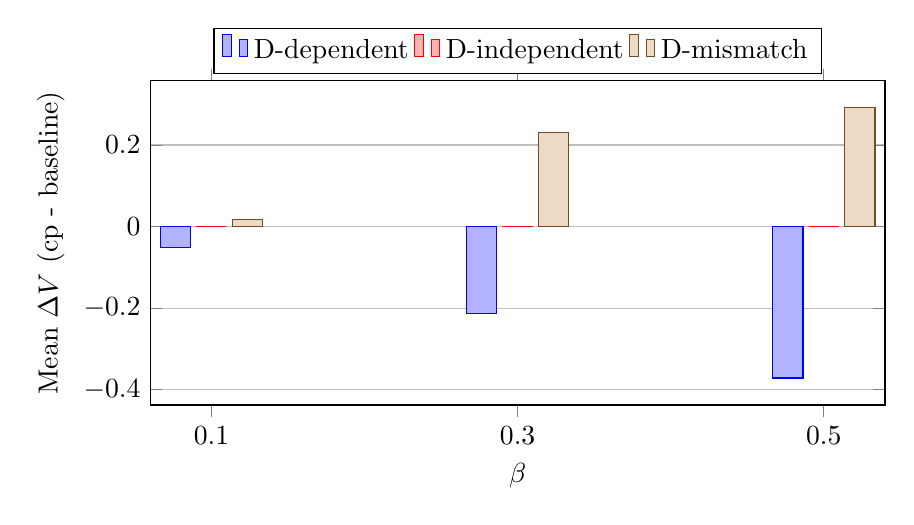
\begin{tikzpicture}
\begin{axis}[
  ybar,
  bar width=11pt,
  width=0.9\textwidth,
  height=5.7cm,
  xlabel={$\beta$},
  ylabel={Mean $\Delta V$ (cp - baseline)},
  symbolic x coords={0.1,0.3,0.5},
  xtick=data,
  legend style={at={(0.5,1.02)},anchor=south,legend columns=3},
  ymajorgrids=true
]
\addplot coordinates {(0.1,-0.0506) (0.3,-0.2123) (0.5,-0.3716)};
\addplot coordinates {(0.1,0.0000) (0.3,0.0000) (0.5,0.0000)};
\addplot coordinates {(0.1,0.0167) (0.3,0.2302) (0.5,0.2914)};
\legend{D-dependent,D-independent,D-mismatch}
\end{axis}
\end{tikzpicture}
\caption{Mean violation-rate difference across 45 samples per condition and beta.}
\label{fig:vdiff}
\end{figure}

\begin{figure}[t]
\centering
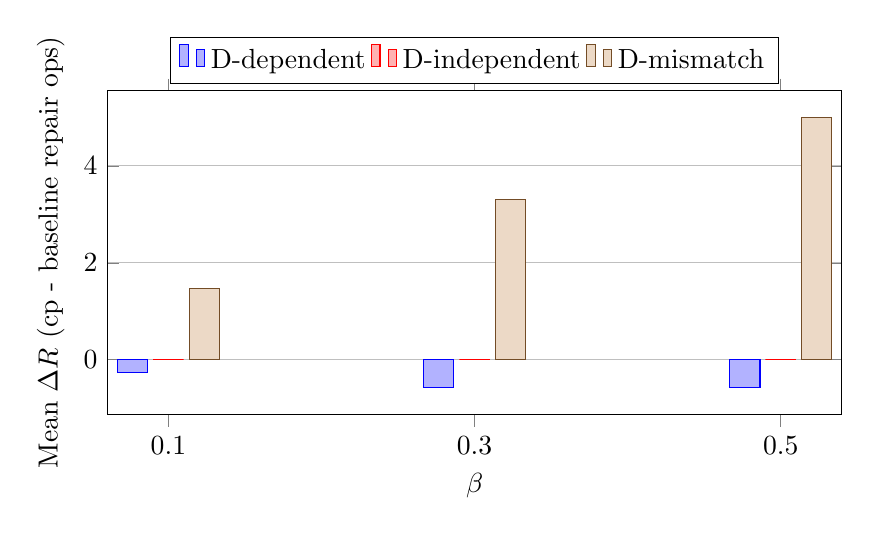
\begin{tikzpicture}
\begin{axis}[
  ybar,
  bar width=11pt,
  width=0.9\textwidth,
  height=5.7cm,
  xlabel={$\beta$},
  ylabel={Mean $\Delta R$ (cp - baseline repair ops)},
  symbolic x coords={0.1,0.3,0.5},
  xtick=data,
  legend style={at={(0.5,1.02)},anchor=south,legend columns=3},
  ymajorgrids=true
]
\addplot coordinates {(0.1,-0.2667) (0.3,-0.5778) (0.5,-0.5778)};
\addplot coordinates {(0.1,0.0000) (0.3,0.0000) (0.5,0.0000)};
\addplot coordinates {(0.1,1.4667) (0.3,3.3111) (0.5,5.0000)};
\legend{D-dependent,D-independent,D-mismatch}
\end{axis}
\end{tikzpicture}
\caption{Mean repair-op difference across 45 samples per condition and beta.}
\label{fig:rdiff}
\end{figure}

\subsection{Pass/fail}
From `cp\_consistency\_report.json` at \(\beta=0.3\): all criteria pass.
D-dependent improves on both metrics; D-mismatch degrades on both metrics; D-independent remains exactly equivalent.

\section{Discussion}
The central empirical pattern is conditional, not universal. In D-dependent settings, coupled propagation lowers violation rate and repair cost relative to the uncoupled baseline. This indicates that when dependency structure is directionally correct, one operator decision can maintain broader state coherence with fewer cleanup actions.

The mismatch results are equally important: sign-inverted dependency matrices increase both violation rate and repair cost. This provides a falsifiable failure mode rather than a one-sided success narrative. In operational terms, cp should be treated as a structure-sensitive mechanism, not as a default improvement over uncoupled updates.

From a system-design perspective, the findings support the original interface hypothesis: LLM-side \((\sigma/\delta,\text{target})\) selection can remain unchanged while dependency handling is implemented client-side. This keeps semantic decision and deterministic state mechanics separated, consistent with the broader NRR design philosophy under tested conditions.

\section{Limitations}
\begin{itemize}
  \item \textbf{Repair cap}: Repair search uses \texttt{max\_repair\_ops=30}. In D-mismatch, cap-hitting cases exist, so reported \(\Delta R\) can be a lower bound on degradation magnitude.
  \item \textbf{Zero-movement handling}: The protocol counts near-zero movement (\(|\Delta w|\le\) tolerance) as violation. This is intentionally conservative and can slightly overcount violations in clipping-saturation turns.
  \item \textbf{Independent-case edge metric}: In D-independent, \(A_{\text{eval}}=0\) implies zero edge opportunities. Therefore violation-rate values in this condition are bookkeeping outputs, while strict trajectory equality is the substantive check.
\end{itemize}

\section{Conclusion}
NRR-Coupled extends the Transfer-style client update with dependency propagation while keeping the LLM interface fixed. Using dependency-consistency metrics, the method shows conditional benefits: improved coherence and lower repair burden when dependency signs are correct, and measurable degradation when they are wrong. The contribution is therefore bounded and falsifiable: cp is useful under validated dependency structure, and unsafe under mis-specified structure.

\section{Reproducibility}
Artifacts:
\begin{itemize}
  \item specification document: `spec/nrr-coupled\_spec.md`
  \item simulation script: `repro/coupled\_state\_sim.py`
  \item reproducibility guide: `repro/README.md`
  \item result tables in `repro/results/cp\_consistency\_*.csv`
  \item contract check in `repro/results/cp\_consistency\_report.json`
\end{itemize}

Main run:
\begin{lstlisting}
python3 repro/coupled_state_sim.py --outdir repro/results
\end{lstlisting}

\section*{Acknowledgments}

The author gratefully acknowledges the support of large language
models---including Claude (Anthropic), ChatGPT and Codex (OpenAI), and Gemini (Google)---for assistance in linguistic refinement,
LaTeX formatting, and general proofreading support during the
preparation of this manuscript.
All concepts, arguments, and conclusions remain solely the
responsibility of the author.

\begin{thebibliography}{99}
\bibitem{saito2025nrr}
Saito, K. (2025).
\textit{NRR-Core: Non-Resolution Reasoning as a Computational Framework for Contextual Identity and Ambiguity Preservation}.
arXiv:2512.13478.

\bibitem{saito2026phi}
Saito, K. (2026).
\textit{NRR-Phi: Text-to-State Mapping for Ambiguity Preservation in LLM Inference}.
arXiv:2601.19933.

\bibitem{saito2026transfer}
Saito, K. (2026).
\textit{NRR-Transfer: Cross-Domain Transfer of Phase 1.5 Operators Under Fixed Interface Constraints}.
Unpublished manuscript.
\end{thebibliography}

\end{document}
